\section{Q1补充模态组合评价}\label{app:q1_modality}
本附录给出不同模态组合的辅助评价结果，与正文表~\ref{tab:q1_modality_ablation} 的精确数值相对应。正文图~\ref{fig:fig07_q1_alignment_method_comparison} 展示的时序对齐比较和图~\ref{fig:fig08_q1_case_source_trace} 展示的典型样本来源追踪均已移至问题一正文。

\begin{figure}[htbp]
    \centering
    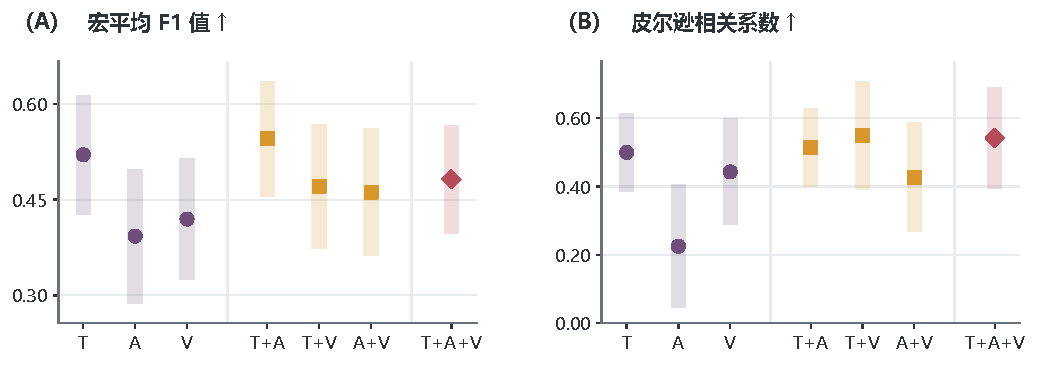
\includegraphics[width=0.98\textwidth]{figures/q1/figA1_q1_modality_combination_ablation.pdf}
    \caption{不同模态组合的辅助评价结果。点表示均值，独立的半透明区间表示均值上下一个样本标准差；圆形、方形和菱形分别表示单模态、双模态和三模态组合。}
    \label{fig:figA1_q1_modality_combination_ablation}
\end{figure}
